\chapter{Prototype 2 Visualizations}
\label{prototype2Viz}

\begin{figure}[h!]
\centering
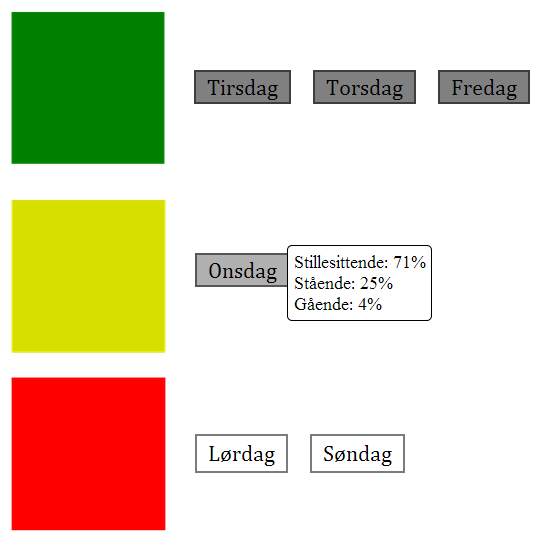
\includegraphics[totalheight=0.5\textheight, angle=-90]{u1Second.png}
\caption[Second version of U1]{Second version of U1.}
\end{figure}

\begin{figure}[h!]
\centering
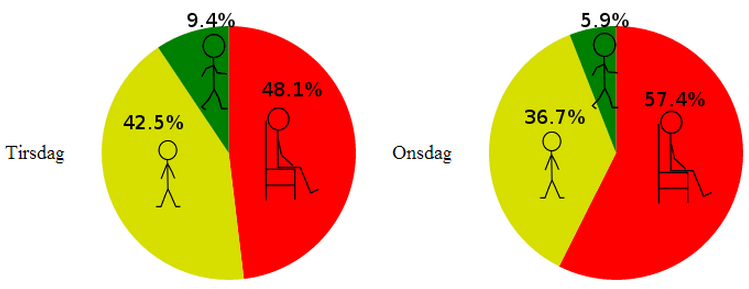
\includegraphics[totalheight=0.35\textheight, angle=90]{f1Second.png}
\caption[Second version of F1]{Second version of F1.}
\end{figure}

\begin{figure}[h!]
\centering
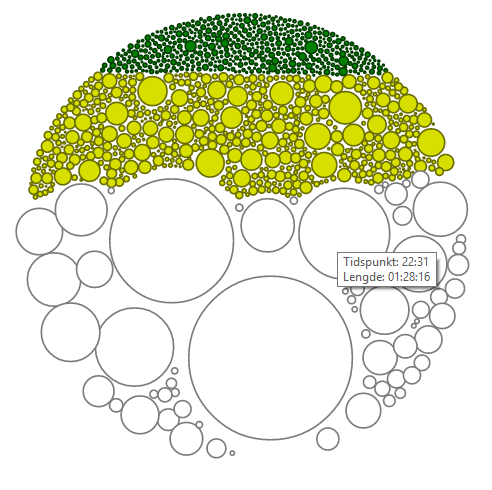
\includegraphics[totalheight=0.5\textheight, angle=-90]{f3Second.png}
\caption[Second version of F3]{Second version of F3.}
\end{figure}

\begin{figure}[h!]
\centering
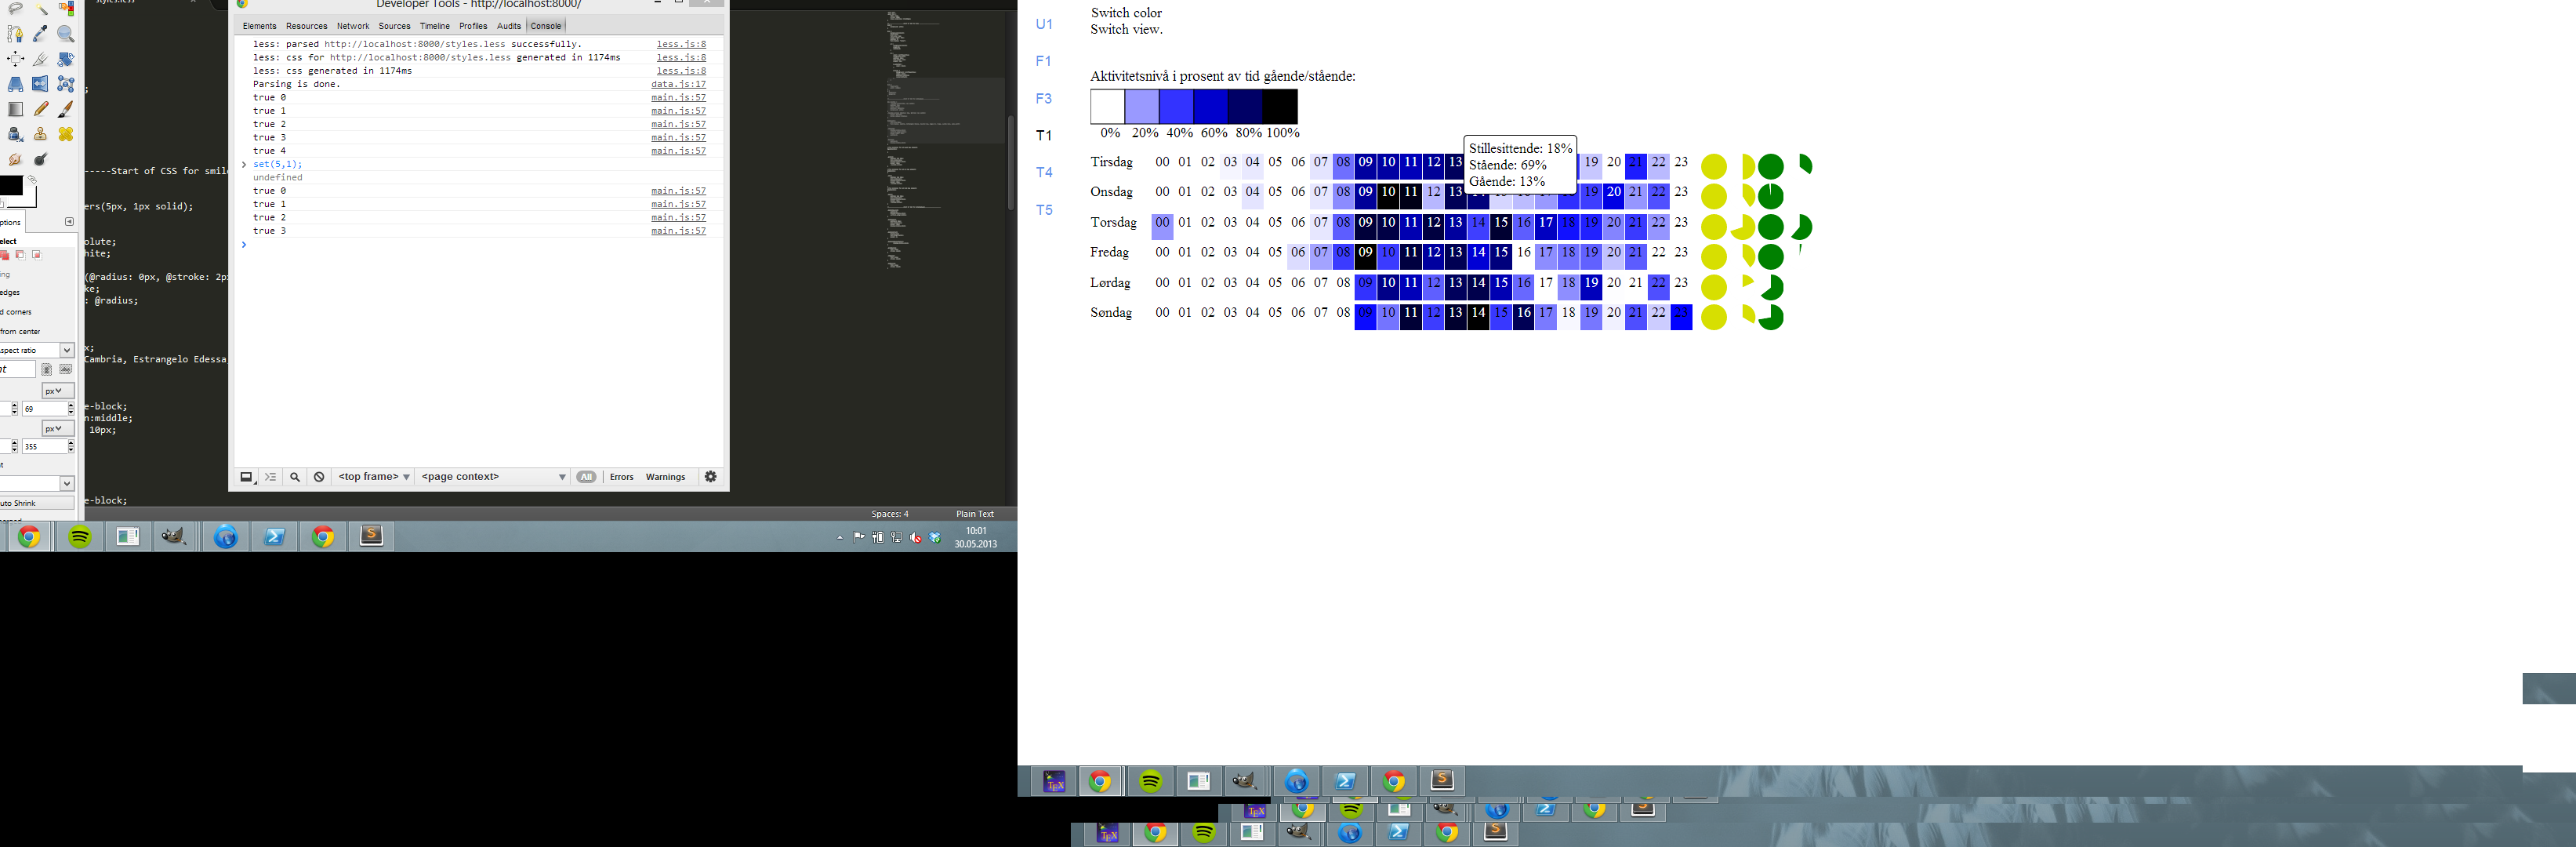
\includegraphics[totalheight=0.35\textheight, angle=90]{t1SecondWeek.png}
\caption[Second version of T1]{Second version of T1 in week overview.}
\end{figure}

\begin{figure}[h!]
\centering
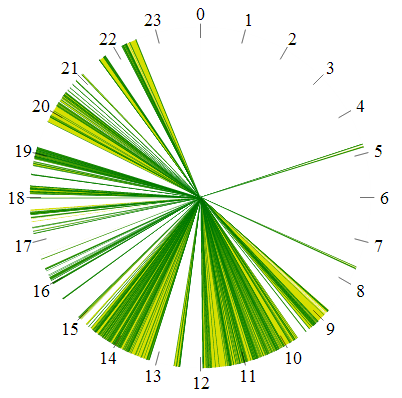
\includegraphics[totalheight=0.5\textheight, angle=-90]{t4Second.png}
\caption[Second version of T4]{Second version of T4.}
\end{figure}

\begin{figure}[h!]
\centering
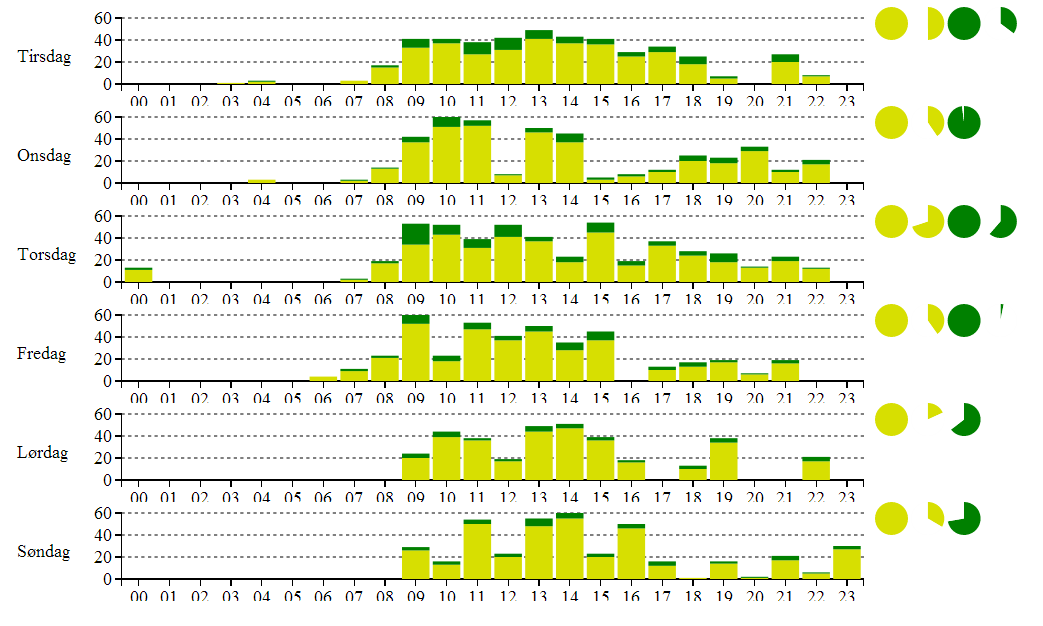
\includegraphics[totalheight=0.5\textheight, angle=90]{t5SecondWeek.png}
\caption[First version of T5]{First version of T5 in week overview.}
\end{figure}
